%% Chapter 5

\cleardoublepage

\chapter{Experiment One}
\label{chp5}

Chapter \ref{chp5} will experiment with a position control system on the NERMLAB. In this experiment a model of the closed-loop position control system will be developed and will be used to predict the response of the NERMLAB. The main purpose of this experiment is not to develop a better position control system but rather demonstrate the concept of changing pole locations and the characteristic of different response to a changing proportional gain. This will be done by looking frequency of oscillation and decay rate of the oscillations of the various responses. Results produced by the NERMLAB will then be compared against the Motorlab, which is the basis of comparison of all experiments in this thesis. 

\section{Mathematical Model of a Closed-Loop Position Control System}

To simply the mathematical formulation the closed-loop current control system is assumed to be much faster than the mechanical dynamics. As a result of this assumption only the mechanical dynamics and controller will be in the model development.  The best way to start the formulation is to begin with a time domain differential equation of the NERMLAB system. The NERMLAB is composed of only an angular mass and viscous friction in this experiment which can be seen in figure \ref{model}.

\begin{figure}[H]
	\tikzset{cross/.style={cross out, draw=black, minimum size=10*(#1-\pgflinewidth), inner sep=0pt, outer sep=0pt},
		%default radius will be 1pt. 
		cross/.default={1.3pt}}
	\begin{center}
		\caption[NERMLAB Model]{NERMLAB Model}
		\label{model}
		\begin{tikzpicture}[scale=2]
		\node[text width=3cm] at (1.1,0.75) {\Large $J$};
		\node[text width=3cm] at (0.5,-0.06) {$b$};
		\draw [thick] (-0.1,-0.16) -- (1.4,-0.16);
		\draw (0,-0.08) node[cross,rotate=2] {};
		\draw (0.1,-0.08) node[cross,rotate=2] {};
		\draw (0.2,-0.08) node[cross,rotate=2] {};
		\draw (0.3,-0.08) node[cross,rotate=2] {};
		\draw (0.4,-0.08) node[cross,rotate=2] {};
		\draw (0.5,-0.08) node[cross,rotate=2] {};
		\draw (0.6,-0.08) node[cross,rotate=2] {};
		\draw (0.7,-0.08) node[cross,rotate=2] {};
		\draw (0.8,-0.08) node[cross,rotate=2] {};
		\draw (0.9,-0.08) node[cross,rotate=2] {};
		\draw (1,-0.08) node[cross,rotate=2] {};
		\draw (1.1,-0.08) node[cross,rotate=2] {};
		\draw (1.2,-0.08) node[cross,rotate=2] {};
		\draw [thick] (0,1.5)  -- (0.2,1.5);
		\draw [thick] (0,0)  -- (0.2,0);
		\draw [thick](0,0) to [out=180, in=180] (0,1.5);
		\draw [thick] (0.2,0) to [out=180, in=180] (0.2,1.5);
		\draw [thick] (0.3,0) to [out=180, in=180] (0.3,1.5);
		\draw [thick] (0.3,0) -- (1.3,0);
		\draw [thick] (0.3,1.5) -- (1.3,1.5);
		\draw [thick] (1.3,0) to [out=0, in=0] (1.3,1.5);
		\draw [thick] (1.3,0) to [out=180, in=180] (1.3,1.5);
		\draw [thick] (1.35,.60) to [out=0, in=0] (1.35,.85);
		\draw [thick] (1.35,.60) to [out=180, in=180] (1.35,.85);
		\draw [->, dashed, thick] (0.6,-0.1) to [out=180, in=180] (0.6,1.6) node[above]{$\theta$}; 
		\draw [->, dashed, thick] (1.2,-0.1) to [out=180, in=180] (1.2,1.6) node[above]{$T$}; 
		\end{tikzpicture}
	\end{center}
\end{figure}

\begin{equation} \label{eq:4.1}
T = k_T i(t) = b \dot \theta(t) + J \ddot \theta(t)
\end{equation}

Taking the Laplace transform of equation \ref{eq:4.1}:
\begin{equation} \label{eq:4.2}
k_T I(s) = (bs + Js^2)\theta(s)
\end{equation}

The transfer function can then be developed for $G_m$ from equation \ref{eq:4.2}.
\begin{equation}
\frac{\theta(s)}{I(s)} = \frac{k_T}{Js^2 + bs}
\end{equation}

As for the controller transfer function, a proportional gain $K_p$ is being used. To further develop the closed loop transfer function, the block diagram in figure \ref{CLCS} can be used. It is as simple as doing a block diagram reduction by merging the blocks in series and then performing a feedback calculation.

% Set up block-diagram shapes
% -------------------------------
\tikzstyle{block} = [draw, rectangle, 
minimum height=3em, minimum width=4em]
\tikzstyle{block2} = [draw, rectangle, 
minimum height=4em, minimum width=7em]
\tikzstyle{sum} = [draw, circle, node distance=1cm]
\tikzstyle{input} = [coordinate]
\tikzstyle{output} = [coordinate]
\tikzstyle{pinstyle} = [pin edge={to-,thin,black}]
% -------------------------------

% Block diagram
% -------------------------------
\begin{figure}[H]
	\begin{center}
		\caption[Block Diagram of Closed Loop Control System]{Closed Loop Control System}
		\label{CLCS}
		
		\begin{tikzpicture}[auto, node distance=2cm,>=latex']
		\node [input, name=input] {};
		\node [sum, right of=input] (sum) {};
		\node [block, right of=sum] (controller) {$G_c$};
		\node [block, right of=controller, node distance=3cm] (system) {$G_m$};
		
		\draw [->] (controller) -- node[name=u] {$I(s)$} (system);
		\node [output, right of=system] (output) {};
		\coordinate [below of=u] (measurements) {};
		
		\draw [draw,->] (input) -- node {$\theta_c(s)$} (sum);
		\draw [->] (sum) -- node {$E(s)$} (controller);
		\draw [->] (system) -- node [name=y] {$\theta$}(output);
		\draw [-] (y) |- (measurements);
		\draw [->] (measurements) -| node [pos=0.99] {$-$} (sum);
		\end{tikzpicture}
	\end{center}
\end{figure}
% -------------------------------

Reducing the blocks in series gives the result:

\begin{equation}
G = G_c G_m = \frac{K_p k_T}{Js^2 + bs}
\end{equation}

The final reduction is performing a feedback calculation:

\begin{equation}
\frac{\theta(s)}{\theta_c(s)} = \frac{G}{1 + G} = \frac{K_p k_T}{Js^2 + bs + K_p k_T}
\end{equation}

% Block diagram
% -------------------------------
\begin{figure}[H]
	\begin{center}
		\caption[Block Diagram Reduction]{Block Diagram Reduction}
		\label{CL}
		
		\begin{tikzpicture}[auto, node distance=2.5cm,>=latex']
		\node [input, name=input] {};
		\node [block2, right of=input] (controller) {$\frac{K_p k_T}{Js^2 + bs + K_p k_T}$};
		\node [output, right of=controller] (output) {};
		\draw [draw,->] (input) -- node {$\theta_c(s)$} (controller);
		\draw [->] (controller) -- node {$\theta(s)$} (output);
		
		\end{tikzpicture}
	\end{center}
\end{figure}
% -------------------------------

\section{Experimental Results}

\begin{figure}[H]
	\begin{center}
		\caption[Base Load Inertia Step Responses]{Base Load Inertia Step Responses}
		\label{Unloaded_Inertia_Step}
		% This file was created by matlab2tikz.
%
%The latest updates can be retrieved from
%  http://www.mathworks.com/matlabcentral/fileexchange/22022-matlab2tikz-matlab2tikz
%where you can also make suggestions and rate matlab2tikz.
%
\definecolor{mycolor1}{rgb}{0.00000,0.44700,0.74100}%
\definecolor{mycolor2}{rgb}{0.85000,0.32500,0.09800}%
\definecolor{mycolor3}{rgb}{0.92900,0.69400,0.12500}%
\definecolor{mycolor4}{rgb}{0.49400,0.18400,0.55600}%
\definecolor{mycolor5}{rgb}{0.46600,0.67400,0.18800}%
\definecolor{mycolor6}{rgb}{0.30100,0.74500,0.93300}%
\definecolor{mycolor7}{rgb}{0.63500,0.07800,0.18400}%
%
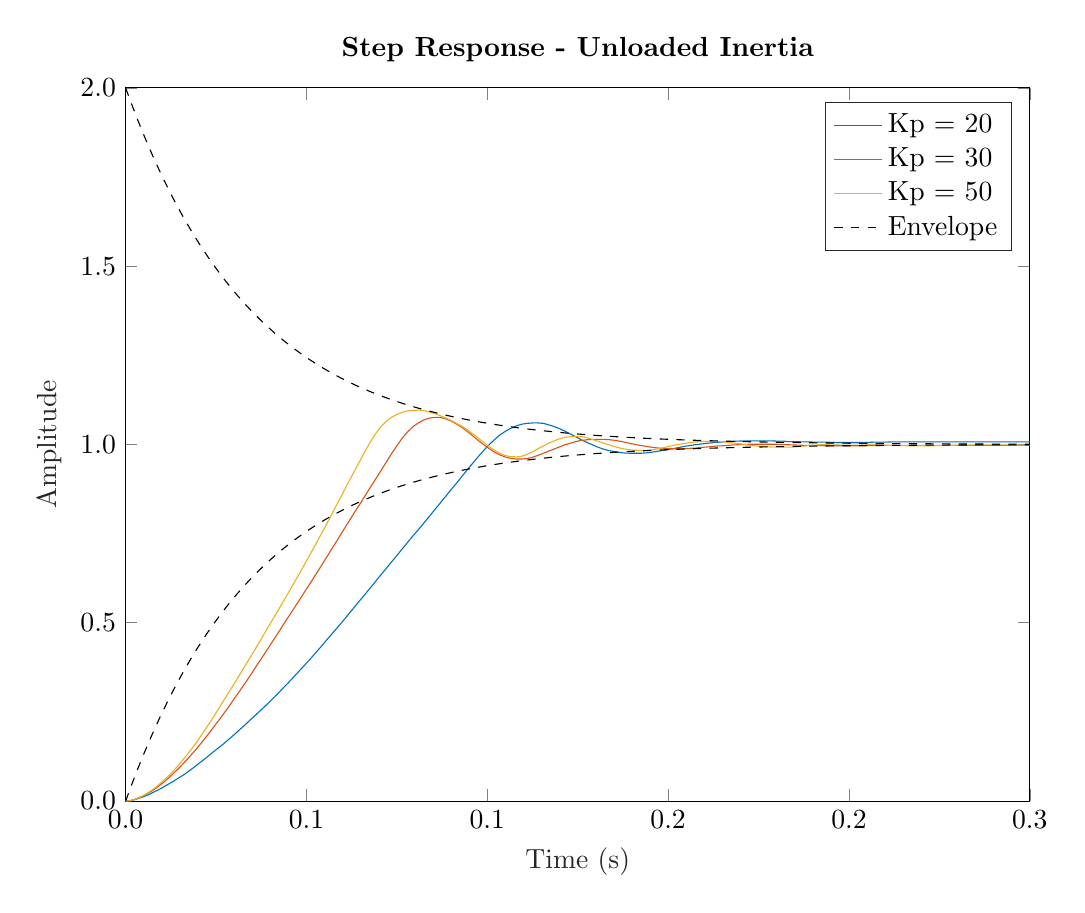
\begin{tikzpicture}

\begin{axis}[%
scaled y ticks = false, 
scaled x ticks = false, 
y tick label style={/pgf/number format/.cd, fixed, fixed zerofill,precision=1},
x tick label style={/pgf/number format/.cd, fixed, fixed zerofill,precision=1},
max space between ticks=50pt,
width=4.521in,
height=3.566in,
at={(0.758in,0.481in)},
scale only axis,
xmin=0,
xmax=0.25,
xlabel style={font=\color{white!15!black}},
xlabel={Time (s)},
ymin=0,
ymax=2,
ylabel style={font=\color{white!15!black}},
ylabel={Amplitude},
axis background/.style={fill=white},
title style={font=\bfseries},
title={Step Response - Unloaded Inertia},
legend style={legend cell align=left, align=left, draw=white!15!black}
]
\addplot [color=mycolor1]
  table[row sep=crcr]{%
-0.00150000001303852	0\\
1.04904174236253e-08	0\\
0.00150002096779644	0.00119679735507816\\
0.00300003145821393	0.00538558792322874\\
0.00450004218146205	0.0107711758464575\\
0.00599993346258998	0.0161567647010088\\
0.00749994395300746	0.0239359457045794\\
0.00899995397776365	0.0311167296022177\\
0.0104999644681811	0.0394943095743656\\
0.0119999749585986	0.0484702922403812\\
0.0134999854490161	0.0574462711811066\\
0.0149999959394336	0.0670206472277641\\
0.0165000073611736	0.0765950307250023\\
0.0180000178515911	0.0879646018147469\\
0.0195000283420086	0.0993341729044914\\
0.0210000388324261	0.111302152276039\\
0.022499930113554	0.123270124197006\\
0.0239999406039715	0.135836496949196\\
0.025499951094389	0.147804468870163\\
0.0269999615848064	0.15977244079113\\
0.0284999720752239	0.172937214374542\\
0.0299999825656414	0.186101987957954\\
0.0314999930560589	0.199865162372589\\
0.0330000035464764	0.213628321886063\\
0.0345000140368938	0.227989882230759\\
0.0360000245273113	0.241753056645393\\
0.0375000350177288	0.256114631891251\\
0.0390000455081463	0.270476192235947\\
0.0404999367892742	0.285436153411865\\
0.0419999472796917	0.300396114587784\\
0.0434999577701092	0.316552877426147\\
0.0449999682605267	0.332111239433289\\
0.0464999787509441	0.348268002271652\\
0.0479999892413616	0.365023195743561\\
0.0494999997317791	0.381179958581924\\
0.0510000102221966	0.397935092449188\\
0.0525000207126141	0.415288656949997\\
0.0540000312030315	0.432642221450806\\
0.055500041693449	0.450594186782837\\
0.056999932974577	0.468546152114868\\
0.0584999434649944	0.485899686813354\\
0.0599999539554119	0.503851652145386\\
0.0614999644458294	0.522402048110962\\
0.0629999712109566	0.540952384471893\\
0.0644999817013741	0.559502720832825\\
0.0659999921917915	0.577454686164856\\
0.067500002682209	0.596005082130432\\
0.0690000131726265	0.614555418491364\\
0.070500023663044	0.63370418548584\\
0.0720000341534615	0.651656150817871\\
0.0734999254345894	0.670206487178802\\
0.0749999359250069	0.688756823539734\\
0.0764999464154243	0.70730721950531\\
0.0779999569058418	0.725857555866241\\
0.0794999673962593	0.744407951831818\\
0.0809999778866768	0.761761486530304\\
0.0824999883770943	0.78031188249588\\
0.0839999988675117	0.798862159252167\\
0.0855000093579292	0.817412614822388\\
0.0870000198483467	0.835962951183319\\
0.0885000303387642	0.85451328754425\\
0.0900000408291817	0.873662054538727\\
0.0914999321103096	0.891614019870758\\
0.0929999426007271	0.910762786865234\\
0.0944999530911446	0.929313123226166\\
0.095999963581562	0.947863459587097\\
0.0974999740719795	0.965815424919128\\
0.098999984562397	0.98316901922226\\
0.100499995052814	0.999325811862946\\
0.102000005543232	1.01368737220764\\
0.103500016033649	1.02685213088989\\
0.105000026524067	1.03702485561371\\
0.106500037014484	1.04540240764618\\
0.107999928295612	1.05198490619659\\
0.10949993878603	1.05677199363709\\
0.110999949276447	1.05916559696198\\
0.112499959766865	1.06036245822906\\
0.113999970257282	1.06036245822906\\
0.1154999807477	1.05916559696198\\
0.116999991238117	1.05497682094574\\
0.118500001728535	1.05018961429596\\
0.120000012218952	1.04420566558838\\
0.12150002270937	1.03702485561371\\
0.123000033199787	1.02924561500549\\
0.124499924480915	1.02146649360657\\
0.125999942421913	1.0130889415741\\
0.127499952912331	1.00590813159943\\
0.128999963402748	0.999325811862946\\
0.130499973893166	0.992743372917175\\
0.131999984383583	0.987357795238495\\
0.133499994874001	0.98316901922226\\
0.135000005364418	0.980177044868469\\
0.136500015854836	0.977783381938934\\
0.138000026345253	0.975988209247589\\
0.13950003683567	0.975389838218689\\
0.141000047326088	0.975389838218689\\
0.142499938607216	0.975389838218689\\
0.143999949097633	0.976586580276489\\
0.145499959588051	0.978381812572479\\
0.146999970078468	0.980775356292725\\
0.148499980568886	0.98316901922226\\
0.149999991059303	0.985562562942505\\
0.151500001549721	0.988554537296295\\
0.153000012040138	0.991546511650085\\
0.154500022530556	0.994538545608521\\
0.156000033020973	0.996932148933411\\
0.157500043511391	0.999325811862946\\
0.158999934792519	1.00112092494965\\
0.160499945282936	1.00291609764099\\
0.161999955773354	1.00471138954163\\
0.163499966263771	1.00590813159943\\
0.164999976754189	1.00710499286652\\
0.166499987244606	1.00770330429077\\
0.167999997735024	1.00890016555786\\
0.169500008225441	1.00949847698212\\
0.171000018715858	1.01009690761566\\
0.172500029206276	1.01009690761566\\
0.174000039696693	1.01009690761566\\
0.175500050187111	1.01009690761566\\
0.176999941468239	1.01009690761566\\
0.178499951958656	1.01009690761566\\
0.179999962449074	1.00949847698212\\
0.181499972939491	1.00949847698212\\
0.182999983429909	1.00830173492432\\
0.184499993920326	1.00770330429077\\
0.186000004410744	1.00770330429077\\
0.187500014901161	1.00710499286652\\
0.189000025391579	1.00710499286652\\
0.190500035881996	1.00650656223297\\
0.192000046372414	1.00650656223297\\
0.193499937653542	1.00650656223297\\
0.194999948143959	1.00590813159943\\
0.196499958634377	1.00590813159943\\
0.197999969124794	1.00590813159943\\
0.199499979615211	1.00590813159943\\
0.200999990105629	1.00590813159943\\
0.202500000596046	1.00590813159943\\
0.204000011086464	1.00590813159943\\
0.205500021576881	1.00590813159943\\
0.207000032067299	1.00650656223297\\
0.208500042557716	1.00650656223297\\
0.209999933838844	1.00650656223297\\
0.211499944329262	1.00710499286652\\
0.212999954819679	1.00710499286652\\
0.214499965310097	1.00710499286652\\
0.215999975800514	1.00710499286652\\
0.217499986290932	1.00710499286652\\
0.218999996781349	1.00710499286652\\
0.220500007271767	1.00710499286652\\
0.222000017762184	1.00710499286652\\
0.223500028252602	1.00710499286652\\
0.225000038743019	1.00710499286652\\
0.226500049233437	1.00710499286652\\
0.227999940514565	1.00710499286652\\
0.229499951004982	1.00710499286652\\
0.230999961495399	1.00710499286652\\
0.232499971985817	1.00710499286652\\
0.233999982476234	1.00710499286652\\
0.235499992966652	1.00710499286652\\
0.237000003457069	1.00710499286652\\
0.238500013947487	1.00710499286652\\
0.240000024437904	1.00710499286652\\
0.241500034928322	1.00710499286652\\
0.243000045418739	1.00710499286652\\
0.244499936699867	1.00710499286652\\
0.245999947190285	1.00710499286652\\
0.247499957680702	1.00710499286652\\
0.24899996817112	1.00710499286652\\
0.250499963760376	1.00710499286652\\
0.251999974250793	1.00710499286652\\
0.253499984741211	1.00710499286652\\
0.254999995231628	1.00710499286652\\
0.256500005722046	1.00710499286652\\
0.258000016212463	1.00710499286652\\
0.259500026702881	1.00710499286652\\
0.260999917984009	1.00710499286652\\
0.262499928474426	1.00710499286652\\
0.263999938964844	1.00710499286652\\
0.265499949455261	1.00710499286652\\
0.266999959945679	1.00710499286652\\
0.268499970436096	1.00710499286652\\
0.269999980926514	1.00710499286652\\
0.271499991416931	1.00710499286652\\
0.273000001907349	1.00710499286652\\
0.274500012397766	1.00710499286652\\
0.276000022888184	1.00710499286652\\
0.277500033378601	1.00710499286652\\
0.278999924659729	1.00710499286652\\
0.280499935150146	1.00710499286652\\
0.281999945640564	1.00710499286652\\
0.283499956130981	1.00710499286652\\
0.284999966621399	1.00710499286652\\
};
\addlegendentry{Kp = 20}

\addplot [color=mycolor2]
  table[row sep=crcr]{%
-0.00150000001303852	0\\
1.04904174236253e-08	0\\
0.00150002096779644	0.00179519597440958\\
0.00300003145821393	0.00658238492906094\\
0.00450004218146205	0.0131647698581219\\
0.00599993346258998	0.0209439527243376\\
0.00749994395300746	0.0299199335277081\\
0.00899995397776365	0.0406911075115204\\
0.0104999644681811	0.0526590794324875\\
0.0119999749585986	0.0658238530158997\\
0.0134999854490161	0.0801854208111763\\
0.0149999959394336	0.0951453819870949\\
0.0165000073611736	0.111302152276039\\
0.0180000178515911	0.128057315945625\\
0.0195000283420086	0.145410880446434\\
0.0210000388324261	0.163961231708527\\
0.022499930113554	0.183109983801842\\
0.0239999406039715	0.202857151627541\\
0.025499951094389	0.223202705383301\\
0.0269999615848064	0.243548259139061\\
0.0284999720752239	0.264492213726044\\
0.0299999825656414	0.28663295507431\\
0.0314999930560589	0.308175325393677\\
0.0330000035464764	0.330316066741943\\
0.0345000140368938	0.353055208921433\\
0.0360000245273113	0.376392751932144\\
0.0375000350177288	0.399131923913956\\
0.0390000455081463	0.422469466924667\\
0.0404999367892742	0.445807009935379\\
0.0419999472796917	0.469144552946091\\
0.0434999577701092	0.493080496788025\\
0.0449999682605267	0.516418039798737\\
0.0464999787509441	0.539755582809448\\
0.0479999892413616	0.56309312582016\\
0.0494999997317791	0.587029099464417\\
0.0510000102221966	0.610366642475128\\
0.0525000207126141	0.634302616119385\\
0.0540000312030315	0.658238530158997\\
0.055500041693449	0.682772874832153\\
0.056999932974577	0.70730721950531\\
0.0584999434649944	0.731243193149567\\
0.0599999539554119	0.756375908851624\\
0.0614999644458294	0.78031188249588\\
0.0629999712109566	0.804846167564392\\
0.0644999817013741	0.828782141208649\\
0.0659999921917915	0.852718055248261\\
0.067500002682209	0.877252399921417\\
0.0690000131726265	0.901188373565674\\
0.070500023663044	0.925124287605286\\
0.0720000341534615	0.949658691883087\\
0.0734999254345894	0.973594546318054\\
0.0749999359250069	0.996333777904511\\
0.0764999464154243	1.01787614822388\\
0.0779999569058418	1.03582811355591\\
0.0794999673962593	1.05018961429596\\
0.0809999778866768	1.06096088886261\\
0.0824999883770943	1.06933844089508\\
0.0839999988675117	1.07412552833557\\
0.0855000093579292	1.07592082023621\\
0.0870000198483467	1.07592082023621\\
0.0885000303387642	1.07173204421997\\
0.0900000408291817	1.0657479763031\\
0.0914999321103096	1.05737042427063\\
0.0929999426007271	1.04779601097107\\
0.0944999530911446	1.03642642498016\\
0.095999963581562	1.02386009693146\\
0.0974999740719795	1.01129376888275\\
0.098999984562397	0.999325811862946\\
0.100499995052814	0.988554537296295\\
0.102000005543232	0.978381812572479\\
0.103500016033649	0.970602571964264\\
0.105000026524067	0.964618563652039\\
0.106500037014484	0.961028218269348\\
0.107999928295612	0.959233045578003\\
0.10949993878603	0.959233045578003\\
0.110999949276447	0.960429847240448\\
0.112499959766865	0.964020252227783\\
0.113999970257282	0.969405829906464\\
0.1154999807477	0.975389838218689\\
0.116999991238117	0.981373846530914\\
0.118500001728535	0.987357795238495\\
0.120000012218952	0.99334180355072\\
0.12150002270937	0.999325811862946\\
0.123000033199787	1.00351452827454\\
0.124499924480915	1.00830173492432\\
0.125999942421913	1.01129376888275\\
0.127499952912331	1.0130889415741\\
0.128999963402748	1.01428580284119\\
0.130499973893166	1.01428580284119\\
0.131999984383583	1.01428580284119\\
0.133499994874001	1.01368737220764\\
0.135000005364418	1.01189208030701\\
0.136500015854836	1.00949847698212\\
0.138000026345253	1.00650656223297\\
0.13950003683567	1.00291609764099\\
0.141000047326088	0.999924182891846\\
0.142499938607216	0.996932148933411\\
0.143999949097633	0.994538545608521\\
0.145499959588051	0.992145001888275\\
0.146999970078468	0.99034982919693\\
0.148499980568886	0.989153027534485\\
0.149999991059303	0.988554537296295\\
0.151500001549721	0.987956166267395\\
0.153000012040138	0.987956166267395\\
0.154500022530556	0.987956166267395\\
0.156000033020973	0.989153027534485\\
0.157500043511391	0.98975133895874\\
0.158999934792519	0.991546511650085\\
0.160499945282936	0.992743372917175\\
0.161999955773354	0.99394017457962\\
0.163499966263771	0.995735347270966\\
0.164999976754189	0.996333777904511\\
0.166499987244606	0.997530519962311\\
0.167999997735024	0.998727321624756\\
0.169500008225441	0.999325811862946\\
0.171000018715858	0.999924182891846\\
0.172500029206276	1.0005224943161\\
0.174000039696693	1.0005224943161\\
0.175500050187111	1.0005224943161\\
0.176999941468239	1.0005224943161\\
0.178499951958656	1.0005224943161\\
0.179999962449074	1.0005224943161\\
0.181499972939491	0.999924182891846\\
0.182999983429909	0.999325811862946\\
0.184499993920326	0.998727321624756\\
0.186000004410744	0.9981290102005\\
0.187500014901161	0.997530519962311\\
0.189000025391579	0.997530519962311\\
0.190500035881996	0.996932148933411\\
0.192000046372414	0.996932148933411\\
0.193499937653542	0.996333777904511\\
0.194999948143959	0.996333777904511\\
0.196499958634377	0.996333777904511\\
0.197999969124794	0.996333777904511\\
0.199499979615211	0.996333777904511\\
0.200999990105629	0.996333777904511\\
0.202500000596046	0.996333777904511\\
0.204000011086464	0.996333777904511\\
0.205500021576881	0.996932148933411\\
0.207000032067299	0.996932148933411\\
0.208500042557716	0.997530519962311\\
0.209999933838844	0.997530519962311\\
0.211499944329262	0.997530519962311\\
0.212999954819679	0.997530519962311\\
0.214499965310097	0.997530519962311\\
0.215999975800514	0.997530519962311\\
0.217499986290932	0.997530519962311\\
0.218999996781349	0.997530519962311\\
0.220500007271767	0.997530519962311\\
0.222000017762184	0.997530519962311\\
0.223500028252602	0.997530519962311\\
0.225000038743019	0.997530519962311\\
0.226500049233437	0.997530519962311\\
0.227999940514565	0.997530519962311\\
0.229499951004982	0.997530519962311\\
0.230999961495399	0.997530519962311\\
0.232499971985817	0.997530519962311\\
0.233999982476234	0.997530519962311\\
0.235499992966652	0.997530519962311\\
0.237000003457069	0.997530519962311\\
0.238500013947487	0.997530519962311\\
0.240000024437904	0.997530519962311\\
0.241500034928322	0.997530519962311\\
0.243000045418739	0.997530519962311\\
0.244499936699867	0.997530519962311\\
0.245999947190285	0.997530519962311\\
0.247499957680702	0.997530519962311\\
0.24899996817112	0.997530519962311\\
0.250499963760376	0.997530519962311\\
0.251999974250793	0.997530519962311\\
0.253499984741211	0.997530519962311\\
0.254999995231628	0.997530519962311\\
0.256500005722046	0.997530519962311\\
0.258000016212463	0.997530519962311\\
0.259500026702881	0.997530519962311\\
0.260999917984009	0.997530519962311\\
0.262499928474426	0.997530519962311\\
0.263999938964844	0.997530519962311\\
0.265499949455261	0.997530519962311\\
0.266999959945679	0.997530519962311\\
0.268499970436096	0.997530519962311\\
0.269999980926514	0.997530519962311\\
0.271499991416931	0.997530519962311\\
0.273000001907349	0.997530519962311\\
0.274500012397766	0.997530519962311\\
0.276000022888184	0.997530519962311\\
0.277500033378601	0.997530519962311\\
0.278999924659729	0.997530519962311\\
0.280499935150146	0.997530519962311\\
0.281999945640564	0.997530519962311\\
0.283499956130981	0.997530519962311\\
0.284999966621399	0.997530519962311\\
};
\addlegendentry{Kp = 30}

\addplot [color=mycolor3]
  table[row sep=crcr]{%
-0.00150000001303852	0\\
1.04904174236253e-08	0\\
0.00150002096779644	0.00119679735507816\\
0.00300003145821393	0.00598398642614484\\
0.00450004218146205	0.0131647698581219\\
0.00599993346258998	0.0221407506614923\\
0.00749994395300746	0.0323135294020176\\
0.00899995397776365	0.0442815013229847\\
0.0104999644681811	0.0580446720123291\\
0.0119999749585986	0.0718078389763832\\
0.0134999854490161	0.0879646018147469\\
0.0149999959394336	0.105318158864975\\
0.0165000073611736	0.123868525028229\\
0.0180000178515911	0.143017277121544\\
0.0195000283420086	0.163362830877304\\
0.0210000388324261	0.185503587126732\\
0.022499930113554	0.208242729306221\\
0.0239999406039715	0.231580287218094\\
0.025499951094389	0.255516231060028\\
0.0269999615848064	0.280050575733185\\
0.0284999720752239	0.304584920406342\\
0.0299999825656414	0.329119265079498\\
0.0314999930560589	0.353653609752655\\
0.0330000035464764	0.378786355257034\\
0.0345000140368938	0.403919070959091\\
0.0360000245273113	0.429051846265793\\
0.0375000350177288	0.454782992601395\\
0.0390000455081463	0.480514109134674\\
0.0404999367892742	0.506245255470276\\
0.0419999472796917	0.531976401805878\\
0.0434999577701092	0.558305978775024\\
0.0449999682605267	0.584037125110626\\
0.0464999787509441	0.610965073108673\\
0.0479999892413616	0.637294590473175\\
0.0494999997317791	0.664222478866577\\
0.0510000102221966	0.691748857498169\\
0.0525000207126141	0.719275176525116\\
0.0540000312030315	0.747399926185608\\
0.055500041693449	0.7755246758461\\
0.056999932974577	0.804247796535492\\
0.0584999434649944	0.833569288253784\\
0.0599999539554119	0.862292408943176\\
0.0614999644458294	0.891614019870758\\
0.0629999712109566	0.92033714056015\\
0.0644999817013741	0.948461890220642\\
0.0659999921917915	0.977185010910034\\
0.067500002682209	1.00411295890808\\
0.0690000131726265	1.02864730358124\\
0.070500023663044	1.04899287223816\\
0.0720000341534615	1.0645512342453\\
0.0734999254345894	1.07592082023621\\
0.0749999359250069	1.08429837226868\\
0.0764999464154243	1.09028232097626\\
0.0779999569058418	1.09447121620178\\
0.0794999673962593	1.09566795825958\\
0.0809999778866768	1.09626638889313\\
0.0824999883770943	1.09506952762604\\
0.0839999988675117	1.0908807516098\\
0.0855000093579292	1.08669197559357\\
0.0870000198483467	1.08070802688599\\
0.0885000303387642	1.07412552833557\\
0.0900000408291817	1.06754326820374\\
0.0914999321103096	1.05916559696198\\
0.0929999426007271	1.0507880449295\\
0.0944999530911446	1.04121363162994\\
0.095999963581562	1.02984404563904\\
0.0974999740719795	1.01787614822388\\
0.098999984562397	1.00590813159943\\
0.100499995052814	0.99394017457962\\
0.102000005543232	0.98376739025116\\
0.103500016033649	0.974791407585144\\
0.105000026524067	0.968807399272919\\
0.106500037014484	0.965815424919128\\
0.107999928295612	0.965217053890228\\
0.10949993878603	0.967012226581573\\
0.110999949276447	0.972397863864899\\
0.112499959766865	0.97957855463028\\
0.113999970257282	0.987956166267395\\
0.1154999807477	0.995735347270966\\
0.116999991238117	1.00351452827454\\
0.118500001728535	1.01009690761566\\
0.120000012218952	1.01608097553253\\
0.12150002270937	1.01967132091522\\
0.123000033199787	1.02206492424011\\
0.124499924480915	1.02206492424011\\
0.125999942421913	1.02206492424011\\
0.127499952912331	1.01907289028168\\
0.128999963402748	1.01428580284119\\
0.130499973893166	1.00949847698212\\
0.131999984383583	1.00411295890808\\
0.133499994874001	0.999325811862946\\
0.135000005364418	0.994538545608521\\
0.136500015854836	0.99034982919693\\
0.138000026345253	0.987357795238495\\
0.13950003683567	0.984964191913605\\
0.141000047326088	0.98376739025116\\
0.142499938607216	0.98316901922226\\
0.143999949097633	0.98316901922226\\
0.145499959588051	0.984964191913605\\
0.146999970078468	0.987357795238495\\
0.148499980568886	0.99034982919693\\
0.149999991059303	0.99394017457962\\
0.151500001549721	0.997530519962311\\
0.153000012040138	1.0005224943161\\
0.154500022530556	1.00291609764099\\
0.156000033020973	1.00530982017517\\
0.157500043511391	1.00710499286652\\
0.158999934792519	1.00830173492432\\
0.160499945282936	1.00830173492432\\
0.161999955773354	1.00830173492432\\
0.163499966263771	1.00830173492432\\
0.164999976754189	1.00770330429077\\
0.166499987244606	1.00590813159943\\
0.167999997735024	1.00411295890808\\
0.169500008225441	1.00231778621674\\
0.171000018715858	0.999924182891846\\
0.172500029206276	0.997530519962311\\
0.174000039696693	0.996333777904511\\
0.175500050187111	0.994538545608521\\
0.176999941468239	0.99394017457962\\
0.178499951958656	0.992743372917175\\
0.179999962449074	0.992743372917175\\
0.181499972939491	0.992743372917175\\
0.182999983429909	0.992743372917175\\
0.184499993920326	0.992743372917175\\
0.186000004410744	0.99394017457962\\
0.187500014901161	0.995136976242065\\
0.189000025391579	0.996932148933411\\
0.190500035881996	0.9981290102005\\
0.192000046372414	0.999325811862946\\
0.193499937653542	0.999924182891846\\
0.194999948143959	1.00112092494965\\
0.196499958634377	1.00112092494965\\
0.197999969124794	1.00171935558319\\
0.199499979615211	1.00171935558319\\
0.200999990105629	1.00171935558319\\
0.202500000596046	1.00171935558319\\
0.204000011086464	1.00112092494965\\
0.205500021576881	1.0005224943161\\
0.207000032067299	0.999924182891846\\
0.208500042557716	0.998727321624756\\
0.209999933838844	0.9981290102005\\
0.211499944329262	0.997530519962311\\
0.212999954819679	0.996932148933411\\
0.214499965310097	0.996932148933411\\
0.215999975800514	0.996333777904511\\
0.217499986290932	0.996333777904511\\
0.218999996781349	0.996333777904511\\
0.220500007271767	0.996333777904511\\
0.222000017762184	0.996333777904511\\
0.223500028252602	0.996333777904511\\
0.225000038743019	0.996932148933411\\
0.226500049233437	0.996932148933411\\
0.227999940514565	0.997530519962311\\
0.229499951004982	0.9981290102005\\
0.230999961495399	0.9981290102005\\
0.232499971985817	0.9981290102005\\
0.233999982476234	0.998727321624756\\
0.235499992966652	0.998727321624756\\
0.237000003457069	0.998727321624756\\
0.238500013947487	0.998727321624756\\
0.240000024437904	0.998727321624756\\
0.241500034928322	0.998727321624756\\
0.243000045418739	0.998727321624756\\
0.244499936699867	0.998727321624756\\
0.245999947190285	0.9981290102005\\
0.247499957680702	0.9981290102005\\
0.24899996817112	0.9981290102005\\
0.250499963760376	0.9981290102005\\
0.251999974250793	0.9981290102005\\
0.253499984741211	0.9981290102005\\
0.254999995231628	0.9981290102005\\
0.256500005722046	0.9981290102005\\
0.258000016212463	0.9981290102005\\
0.259500026702881	0.9981290102005\\
0.260999917984009	0.9981290102005\\
0.262499928474426	0.9981290102005\\
0.263999938964844	0.9981290102005\\
0.265499949455261	0.9981290102005\\
0.266999959945679	0.9981290102005\\
0.268499970436096	0.9981290102005\\
0.269999980926514	0.9981290102005\\
0.271499991416931	0.9981290102005\\
0.273000001907349	0.9981290102005\\
0.274500012397766	0.9981290102005\\
0.276000022888184	0.9981290102005\\
0.277500033378601	0.9981290102005\\
0.278999924659729	0.9981290102005\\
0.280499935150146	0.9981290102005\\
0.281999945640564	0.9981290102005\\
0.283499956130981	0.9981290102005\\
0.284999966621399	0.9981290102005\\
};
\addlegendentry{Kp = 50}

\addplot [color=black, dashed]
  table[row sep=crcr]{%
0	0\\
0.00163161179689557	0.0450074139785637\\
0.00326322359379114	0.0879891606440896\\
0.00489483539068671	0.129036410043918\\
0.00652644718758227	0.168236228897328\\
0.00815805898447784	0.205671765275717\\
0.00978967078137341	0.241422424970815\\
0.011421282578269	0.275564039925008\\
0.0130528943751645	0.308169029081062\\
0.0146845061720601	0.339306551992402\\
0.0163161179689557	0.369042655519805\\
0.0179477297658513	0.39744041392564\\
0.0195793415627468	0.424560062662841\\
0.0212109533596424	0.450459126142373\\
0.022842565156538	0.475192539750225\\
0.0244741769534335	0.498812766372725\\
0.0261057887503291	0.521369907677359\\
0.0277374005472247	0.542911810385122\\
0.0293690123441202	0.563484167759831\\
0.0310006241410158	0.583130616529662\\
0.0326322359379114	0.6018928294465\\
0.0342638477348069	0.619810603679436\\
0.0358954595317025	0.636921945229896\\
0.0375270713285981	0.653263149547466\\
0.0391586831254936	0.668868878517407\\
0.0407902949223892	0.68377223398316\\
0.0424219067192848	0.698004827959796\\
0.0440535185161803	0.711596849687337\\
0.0456851303130759	0.724577129666181\\
0.0473167421099715	0.73697320081046\\
0.0489483539068671	0.74881135684904\\
0.0505799657037626	0.760116708098049\\
0.0522115775006582	0.770913234723221\\
0.0538431892975538	0.781223837605043\\
0.0554748010944493	0.791070386914594\\
0.0571064128913449	0.80047376850311\\
0.0587380246882405	0.809453928203674\\
0.060369636485136	0.818029914139\\
0.0620012482820316	0.826219917125061\\
0.0636328600789272	0.834041309256243\\
0.0652644718758227	0.841510680753887\\
0.0668960836727183	0.848643875156378\\
0.0685276954696139	0.855456022925406\\
0.0701593072665094	0.86196157353971\\
0.071790919063405	0.868174326144358\\
0.0734225308603006	0.874107458820582\\
0.0750541426571961	0.879773556538258\\
0.0766857544540917	0.885184637850311\\
0.0783173662509873	0.890352180385681\\
0.0799489780478829	0.895287145194909\\
0.0815805898447784	0.899999999999999\\
0.083212201641674	0.904500741397856\\
0.0848438134385696	0.908798916064408\\
0.0864754252354651	0.912903641004391\\
0.0881070370323607	0.916823622889732\\
0.0897386488292563	0.920567176527571\\
0.0913702606261518	0.924142242497081\\
0.0930018724230474	0.927556403992501\\
0.094633484219943	0.930816902908106\\
0.0962650960168385	0.93393065519924\\
0.0978967078137341	0.93690426555198\\
0.0995283196106297	0.939744041392564\\
0.101159931407525	0.942456006266284\\
0.102791543204421	0.945045912614238\\
0.104423155001316	0.947519253975023\\
0.106054766798212	0.949881276637273\\
0.107686378595108	0.952136990767736\\
0.109317990392003	0.954291181038513\\
0.110949602188899	0.956348416775983\\
0.112581213985794	0.958313061652967\\
0.11421282578269	0.96018928294465\\
0.115844437579585	0.961981060367944\\
0.117476049376481	0.96369219452299\\
0.119107661173377	0.965326314954747\\
0.120739272970272	0.966886887851741\\
0.122370884767168	0.968377223398317\\
0.124002496564063	0.96980048279598\\
0.125634108360959	0.971159684968735\\
0.127265720157854	0.972457712966619\\
0.12889733195475	0.973697320081047\\
0.130528943751645	0.974881135684905\\
0.132160555548541	0.976011670809806\\
0.133792167345437	0.977091323472323\\
0.135423779142332	0.978122383760505\\
0.137055390939228	0.979107038691461\\
0.138687002736123	0.980047376850312\\
0.140318614533019	0.980945392820369\\
0.141950226329914	0.981802991413901\\
0.14358183812681	0.982621991712507\\
0.145213449923706	0.983404130925625\\
0.146845061720601	0.98415106807539\\
0.148476673517497	0.984864387515639\\
0.150108285314392	0.985545602292542\\
0.151739897111288	0.986196157353972\\
0.153371508908183	0.986817432614437\\
0.155003120705079	0.987410745882059\\
0.156634732501975	0.987977355653827\\
0.15826634429887	0.988518463785032\\
0.159897956095766	0.989035218038569\\
0.161529567892661	0.989528714519492\\
0.163161179689557	0.990000000000001\\
0.164792791486452	0.990450074139787\\
0.166424403283348	0.990879891606442\\
0.168056015080244	0.99129036410044\\
0.169687626877139	0.991682362288975\\
0.171319238674035	0.992056717652758\\
0.17295085047093	0.992414224249709\\
0.174582462267826	0.992755640399251\\
0.176214074064721	0.993081690290812\\
0.177845685861617	0.993393065519925\\
0.179477297658513	0.9936904265552\\
0.181108909455408	0.993974404139258\\
0.182740521252304	0.99424560062663\\
0.184372133049199	0.994504591261425\\
0.186003744846095	0.994751925397504\\
0.18763535664299	0.994988127663729\\
0.189266968439886	0.995213699076775\\
0.190898580236782	0.995429118103853\\
0.192530192033677	0.9956348416776\\
0.194161803830573	0.995831306165298\\
0.195793415627468	0.996018928294466\\
0.197425027424364	0.996198106036796\\
0.199056639221259	0.996369219452301\\
0.200688251018155	0.996532631495476\\
0.20231986281505	0.996688688785176\\
0.203951474611946	0.996837722339833\\
0.205583086408842	0.996980048279599\\
0.207214698205737	0.997115968496875\\
0.208846310002633	0.997245771296663\\
0.210477921799528	0.997369732008106\\
0.212109533596424	0.997488113568492\\
0.213741145393319	0.997601167080982\\
0.215372757190215	0.997709132347234\\
0.217004368987111	0.997812238376052\\
0.218635980784006	0.997910703869148\\
0.220267592580902	0.998004737685033\\
0.221899204377797	0.998094539282038\\
0.223530816174693	0.998180299141392\\
0.225162427971588	0.998262199171252\\
0.226794039768484	0.998340413092564\\
0.22842565156538	0.99841510680754\\
0.230057263362275	0.998486438751565\\
0.231688875159171	0.998554560229256\\
0.233320486956066	0.998619615735399\\
0.234952098752962	0.998681743261445\\
0.236583710549857	0.998741074588207\\
0.238215322346753	0.998797735565384\\
0.239846934143649	0.998851846378505\\
0.241478545940544	0.998903521803858\\
0.24311015773744	0.998952871451951\\
0.244741769534335	0.999000000000001\\
0.246373381331231	0.99904500741398\\
0.248004993128126	0.999087989160646\\
0.249636604925022	0.999129036410046\\
0.251268216721918	0.999168236228899\\
0.252899828518813	0.999205671765278\\
0.254531440315709	0.999241422424973\\
0.256163052112604	0.999275564039927\\
0.2577946639095	0.999308169029083\\
0.259426275706395	0.999339306551994\\
0.261057887503291	0.999369042655522\\
0.262689499300187	0.999397440413927\\
0.264321111097082	0.999424560062665\\
0.265952722893978	0.999450459126144\\
0.267584334690873	0.999475192539752\\
0.269215946487769	0.999498812766375\\
0.270847558284664	0.999521369907679\\
0.27247917008156	0.999542911810387\\
0.274110781878456	0.999563484167762\\
0.275742393675351	0.999583130616531\\
0.277374005472247	0.999601892829448\\
0.279005617269142	0.999619810603681\\
0.280637229066038	0.999636921945232\\
0.282268840862933	0.999653263149549\\
0.283900452659829	0.999668868878519\\
0.285532064456724	0.999683772233985\\
0.28716367625362	0.999698004827962\\
0.288795288050516	0.999711596849689\\
0.290426899847411	0.999724577129668\\
0.292058511644307	0.999736973200812\\
0.293690123441202	0.999748811356851\\
0.295321735238098	0.9997601167081\\
0.296953347034993	0.999770913234725\\
0.298584958831889	0.999781223837607\\
0.300216570628785	0.999791070386916\\
0.30184818242568	0.999800473768505\\
0.303479794222576	0.999809453928206\\
0.305111406019471	0.999818029914141\\
0.306743017816367	0.999826219917127\\
0.308374629613262	0.999834041309258\\
0.310006241410158	0.999841510680756\\
0.311637853207054	0.999848643875158\\
0.313269465003949	0.999855456022927\\
0.314901076800845	0.999861961573541\\
0.31653268859774	0.999868174326146\\
0.318164300394636	0.999874107458822\\
};
\addlegendentry{Envelope}

\addplot [color=black, dashed, forget plot]
  table[row sep=crcr]{%
0	2\\
0.00163161179689557	1.95499258602144\\
0.00326322359379114	1.91201083935591\\
0.00489483539068671	1.87096358995608\\
0.00652644718758227	1.83176377110267\\
0.00815805898447784	1.79432823472428\\
0.00978967078137341	1.75857757502919\\
0.011421282578269	1.72443596007499\\
0.0130528943751645	1.69183097091894\\
0.0146845061720601	1.6606934480076\\
0.0163161179689557	1.6309573444802\\
0.0179477297658513	1.60255958607436\\
0.0195793415627468	1.57543993733716\\
0.0212109533596424	1.54954087385763\\
0.022842565156538	1.52480746024978\\
0.0244741769534335	1.50118723362727\\
0.0261057887503291	1.47863009232264\\
0.0277374005472247	1.45708818961488\\
0.0293690123441202	1.43651583224017\\
0.0310006241410158	1.41686938347034\\
0.0326322359379114	1.3981071705535\\
0.0342638477348069	1.38018939632056\\
0.0358954595317025	1.3630780547701\\
0.0375270713285981	1.34673685045253\\
0.0391586831254936	1.33113112148259\\
0.0407902949223892	1.31622776601684\\
0.0424219067192848	1.3019951720402\\
0.0440535185161803	1.28840315031266\\
0.0456851303130759	1.27542287033382\\
0.0473167421099715	1.26302679918954\\
0.0489483539068671	1.25118864315096\\
0.0505799657037626	1.23988329190195\\
0.0522115775006582	1.22908676527678\\
0.0538431892975538	1.21877616239496\\
0.0554748010944493	1.20892961308541\\
0.0571064128913449	1.19952623149689\\
0.0587380246882405	1.19054607179633\\
0.060369636485136	1.181970085861\\
0.0620012482820316	1.17378008287494\\
0.0636328600789272	1.16595869074376\\
0.0652644718758227	1.15848931924611\\
0.0668960836727183	1.15135612484362\\
0.0685276954696139	1.14454397707459\\
0.0701593072665094	1.13803842646029\\
0.071790919063405	1.13182567385564\\
0.0734225308603006	1.12589254117942\\
0.0750541426571961	1.12022644346174\\
0.0766857544540917	1.11481536214969\\
0.0783173662509873	1.10964781961432\\
0.0799489780478829	1.10471285480509\\
0.0815805898447784	1.1\\
0.083212201641674	1.09549925860214\\
0.0848438134385696	1.09120108393559\\
0.0864754252354651	1.08709635899561\\
0.0881070370323607	1.08317637711027\\
0.0897386488292563	1.07943282347243\\
0.0913702606261518	1.07585775750292\\
0.0930018724230474	1.0724435960075\\
0.094633484219943	1.06918309709189\\
0.0962650960168385	1.06606934480076\\
0.0978967078137341	1.06309573444802\\
0.0995283196106297	1.06025595860744\\
0.101159931407525	1.05754399373372\\
0.102791543204421	1.05495408738576\\
0.104423155001316	1.05248074602498\\
0.106054766798212	1.05011872336273\\
0.107686378595108	1.04786300923226\\
0.109317990392003	1.04570881896149\\
0.110949602188899	1.04365158322402\\
0.112581213985794	1.04168693834703\\
0.11421282578269	1.03981071705535\\
0.115844437579585	1.03801893963206\\
0.117476049376481	1.03630780547701\\
0.119107661173377	1.03467368504525\\
0.120739272970272	1.03311311214826\\
0.122370884767168	1.03162277660168\\
0.124002496564063	1.03019951720402\\
0.125634108360959	1.02884031503127\\
0.127265720157854	1.02754228703338\\
0.12889733195475	1.02630267991895\\
0.130528943751645	1.0251188643151\\
0.132160555548541	1.02398832919019\\
0.133792167345437	1.02290867652768\\
0.135423779142332	1.02187761623949\\
0.137055390939228	1.02089296130854\\
0.138687002736123	1.01995262314969\\
0.140318614533019	1.01905460717963\\
0.141950226329914	1.0181970085861\\
0.14358183812681	1.01737800828749\\
0.145213449923706	1.01659586907437\\
0.146845061720601	1.01584893192461\\
0.148476673517497	1.01513561248436\\
0.150108285314392	1.01445439770746\\
0.151739897111288	1.01380384264603\\
0.153371508908183	1.01318256738556\\
0.155003120705079	1.01258925411794\\
0.156634732501975	1.01202264434617\\
0.15826634429887	1.01148153621497\\
0.159897956095766	1.01096478196143\\
0.161529567892661	1.01047128548051\\
0.163161179689557	1.01\\
0.164792791486452	1.00954992586021\\
0.166424403283348	1.00912010839356\\
0.168056015080244	1.00870963589956\\
0.169687626877139	1.00831763771103\\
0.171319238674035	1.00794328234724\\
0.17295085047093	1.00758577575029\\
0.174582462267826	1.00724435960075\\
0.176214074064721	1.00691830970919\\
0.177845685861617	1.00660693448007\\
0.179477297658513	1.0063095734448\\
0.181108909455408	1.00602559586074\\
0.182740521252304	1.00575439937337\\
0.184372133049199	1.00549540873857\\
0.186003744846095	1.0052480746025\\
0.18763535664299	1.00501187233627\\
0.189266968439886	1.00478630092322\\
0.190898580236782	1.00457088189615\\
0.192530192033677	1.0043651583224\\
0.194161803830573	1.0041686938347\\
0.195793415627468	1.00398107170553\\
0.197425027424364	1.0038018939632\\
0.199056639221259	1.0036307805477\\
0.200688251018155	1.00346736850452\\
0.20231986281505	1.00331131121482\\
0.203951474611946	1.00316227766017\\
0.205583086408842	1.0030199517204\\
0.207214698205737	1.00288403150313\\
0.208846310002633	1.00275422870334\\
0.210477921799528	1.00263026799189\\
0.212109533596424	1.00251188643151\\
0.213741145393319	1.00239883291902\\
0.215372757190215	1.00229086765277\\
0.217004368987111	1.00218776162395\\
0.218635980784006	1.00208929613085\\
0.220267592580902	1.00199526231497\\
0.221899204377797	1.00190546071796\\
0.223530816174693	1.00181970085861\\
0.225162427971588	1.00173780082875\\
0.226794039768484	1.00165958690744\\
0.22842565156538	1.00158489319246\\
0.230057263362275	1.00151356124843\\
0.231688875159171	1.00144543977074\\
0.233320486956066	1.0013803842646\\
0.234952098752962	1.00131825673855\\
0.236583710549857	1.00125892541179\\
0.238215322346753	1.00120226443462\\
0.239846934143649	1.0011481536215\\
0.241478545940544	1.00109647819614\\
0.24311015773744	1.00104712854805\\
0.244741769534335	1.001\\
0.246373381331231	1.00095499258602\\
0.248004993128126	1.00091201083935\\
0.249636604925022	1.00087096358995\\
0.251268216721918	1.0008317637711\\
0.252899828518813	1.00079432823472\\
0.254531440315709	1.00075857757503\\
0.256163052112604	1.00072443596007\\
0.2577946639095	1.00069183097092\\
0.259426275706395	1.00066069344801\\
0.261057887503291	1.00063095734448\\
0.262689499300187	1.00060255958607\\
0.264321111097082	1.00057543993734\\
0.265952722893978	1.00054954087386\\
0.267584334690873	1.00052480746025\\
0.269215946487769	1.00050118723363\\
0.270847558284664	1.00047863009232\\
0.27247917008156	1.00045708818961\\
0.274110781878456	1.00043651583224\\
0.275742393675351	1.00041686938347\\
0.277374005472247	1.00039810717055\\
0.279005617269142	1.00038018939632\\
0.280637229066038	1.00036307805477\\
0.282268840862933	1.00034673685045\\
0.283900452659829	1.00033113112148\\
0.285532064456724	1.00031622776602\\
0.28716367625362	1.00030199517204\\
0.288795288050516	1.00028840315031\\
0.290426899847411	1.00027542287033\\
0.292058511644307	1.00026302679919\\
0.293690123441202	1.00025118864315\\
0.295321735238098	1.0002398832919\\
0.296953347034993	1.00022908676528\\
0.298584958831889	1.00021877616239\\
0.300216570628785	1.00020892961308\\
0.30184818242568	1.0001995262315\\
0.303479794222576	1.00019054607179\\
0.305111406019471	1.00018197008586\\
0.306743017816367	1.00017378008287\\
0.308374629613262	1.00016595869074\\
0.310006241410158	1.00015848931924\\
0.311637853207054	1.00015135612484\\
0.313269465003949	1.00014454397707\\
0.314901076800845	1.00013803842646\\
0.31653268859774	1.00013182567385\\
0.318164300394636	1.00012589254118\\
};
\addplot [color=mycolor4, forget plot]
  table[row sep=crcr]{%
0.1865	0\\
};
\addplot [color=mycolor5, forget plot]
  table[row sep=crcr]{%
0.1865	0.00844449250782346\\
};
\addplot [color=mycolor6, forget plot]
  table[row sep=crcr]{%
0.1865	0.0326390378370615\\
};
\addplot [color=mycolor7, forget plot]
  table[row sep=crcr]{%
0.1865	0.070795361160574\\
};
\addplot [color=mycolor1, forget plot]
  table[row sep=crcr]{%
0.1865	0.121050302681586\\
};
\addplot [color=mycolor2, forget plot]
  table[row sep=crcr]{%
0.1865	0.18150339763937\\
};
\addplot [color=mycolor3, forget plot]
  table[row sep=crcr]{%
0.1865	0.250251770195329\\
};
\addplot [color=mycolor4, forget plot]
  table[row sep=crcr]{%
0.1865	0.325421997140081\\
};
\addplot [color=mycolor5, forget plot]
  table[row sep=crcr]{%
0.1865	0.405198678038266\\
};
\addplot [color=mycolor6, forget plot]
  table[row sep=crcr]{%
0.1865	0.487849526386252\\
};
\addplot [color=mycolor7, forget plot]
  table[row sep=crcr]{%
0.1865	0.571746870541154\\
};
\addplot [color=mycolor1, forget plot]
  table[row sep=crcr]{%
0.1865	0.655385522685854\\
};
\addplot [color=mycolor2, forget plot]
  table[row sep=crcr]{%
0.1865	0.737397038179366\\
};
\addplot [color=mycolor3, forget plot]
  table[row sep=crcr]{%
0.1865	0.816560445716052\\
};
\addplot [color=mycolor4, forget plot]
  table[row sep=crcr]{%
0.1865	0.891809580343755\\
};
\addplot [color=mycolor5, forget plot]
  table[row sep=crcr]{%
0.1865	0.962237196278379\\
};
\addplot [color=mycolor6, forget plot]
  table[row sep=crcr]{%
0.1865	1.02709607444729\\
};
\addplot [color=mycolor7, forget plot]
  table[row sep=crcr]{%
0.1865	1.08579737077046\\
};
\addplot [color=mycolor1, forget plot]
  table[row sep=crcr]{%
0.1865	1.13790647543841\\
};
\addplot [color=mycolor2, forget plot]
  table[row sep=crcr]{%
0.1865	1.18313667106716\\
};
\addplot [color=mycolor3, forget plot]
  table[row sep=crcr]{%
0.1865	1.2213408888925\\
};
\addplot [color=mycolor4, forget plot]
  table[row sep=crcr]{%
0.1865	1.25250186747906\\
};
\addplot [color=mycolor5, forget plot]
  table[row sep=crcr]{%
0.1865	1.27672101820115\\
};
\addplot [color=mycolor6, forget plot]
  table[row sep=crcr]{%
0.1865	1.29420629649187\\
};
\addplot [color=mycolor7, forget plot]
  table[row sep=crcr]{%
0.1865	1.30525936808612\\
};
\addplot [color=mycolor1, forget plot]
  table[row sep=crcr]{%
0.1865	1.31026234576118\\
};
\addplot [color=mycolor2, forget plot]
  table[row sep=crcr]{%
0.1865	1.30966435498146\\
};
\addplot [color=mycolor3, forget plot]
  table[row sep=crcr]{%
0.1865	1.30396816696269\\
};
\addplot [color=mycolor4, forget plot]
  table[row sep=crcr]{%
0.1865	1.29371711556298\\
};
\addplot [color=mycolor5, forget plot]
  table[row sep=crcr]{%
0.1865	1.27948249064539\\
};
\addplot [color=mycolor6, forget plot]
  table[row sep=crcr]{%
0.1865	1.26185157568056\\
};
\addplot [color=mycolor7, forget plot]
  table[row sep=crcr]{%
0.1865	1.24141647188051\\
};
\addplot [color=mycolor1, forget plot]
  table[row sep=crcr]{%
0.1865	1.2187638255513\\
};
\addplot [color=mycolor2, forget plot]
  table[row sep=crcr]{%
0.1865	1.19446555006179\\
};
\addplot [color=mycolor3, forget plot]
  table[row sep=crcr]{%
0.1865	1.16907060923942\\
};
\addplot [color=mycolor4, forget plot]
  table[row sep=crcr]{%
0.1865	1.14309790547017\\
};
\addplot [color=mycolor5, forget plot]
  table[row sep=crcr]{%
0.1865	1.11703029359681\\
};
\addplot [color=mycolor6, forget plot]
  table[row sep=crcr]{%
0.1865	1.09130972112735\\
};
\addplot [color=mycolor7, forget plot]
  table[row sep=crcr]{%
0.1865	1.0663334764863\\
};
\addplot [color=mycolor1, forget plot]
  table[row sep=crcr]{%
0.1865	1.04245151021759\\
};
\addplot [color=mycolor2, forget plot]
  table[row sep=crcr]{%
0.1865	1.01996477928922\\
};
\addplot [color=mycolor3, forget plot]
  table[row sep=crcr]{%
0.1865	0.999124552017514\\
};
\addplot [color=mycolor4, forget plot]
  table[row sep=crcr]{%
0.1865	0.980132600648729\\
};
\addplot [color=mycolor5, forget plot]
  table[row sep=crcr]{%
0.1865	0.963142200290288\\
};
\addplot [color=mycolor6, forget plot]
  table[row sep=crcr]{%
0.1865	0.948259846625934\\
};
\addplot [color=mycolor7, forget plot]
  table[row sep=crcr]{%
0.1865	0.935547600597909\\
};
\addplot [color=mycolor1, forget plot]
  table[row sep=crcr]{%
0.1865	0.925025965889495\\
};
\addplot [color=mycolor2, forget plot]
  table[row sep=crcr]{%
0.1865	0.916677204464543\\
};
\addplot [color=mycolor3, forget plot]
  table[row sep=crcr]{%
0.1865	0.910448996470575\\
};
\addplot [color=mycolor4, forget plot]
  table[row sep=crcr]{%
0.1865	0.906258353328052\\
};
\addplot [color=mycolor5, forget plot]
  table[row sep=crcr]{%
0.1865	0.903995696639653\\
};
\addplot [color=mycolor6, forget plot]
  table[row sep=crcr]{%
0.1865	0.903529020482502\\
};
\addplot [color=mycolor7, forget plot]
  table[row sep=crcr]{%
0.1865	0.904708060512913\\
};
\addplot [color=mycolor1, forget plot]
  table[row sep=crcr]{%
0.1865	0.907368399937239\\
};
\addplot [color=mycolor2, forget plot]
  table[row sep=crcr]{%
0.1865	0.911335449607122\\
};
\addplot [color=mycolor3, forget plot]
  table[row sep=crcr]{%
0.1865	0.916428247111754\\
};
\addplot [color=mycolor4, forget plot]
  table[row sep=crcr]{%
0.1865	0.9224630276011\\
};
\addplot [color=mycolor5, forget plot]
  table[row sep=crcr]{%
0.1865	0.92925652702987\\
};
\addplot [color=mycolor6, forget plot]
  table[row sep=crcr]{%
0.1865	0.936628986421665\\
};
\addplot [color=mycolor7, forget plot]
  table[row sep=crcr]{%
0.1865	0.944406833488752\\
};
\addplot [color=mycolor1, forget plot]
  table[row sep=crcr]{%
0.1865	0.95242502539183\\
};
\addplot [color=mycolor2, forget plot]
  table[row sep=crcr]{%
0.1865	0.960529043487441\\
};
\addplot [color=mycolor3, forget plot]
  table[row sep=crcr]{%
0.1865	0.968576537504592\\
};
\addplot [color=mycolor4, forget plot]
  table[row sep=crcr]{%
0.1865	0.976438622648586\\
};
\addplot [color=mycolor5, forget plot]
  table[row sep=crcr]{%
0.1865	0.984000838595247\\
};
\addplot [color=mycolor6, forget plot]
  table[row sep=crcr]{%
0.1865	0.991163784174061\\
};
\addplot [color=mycolor7, forget plot]
  table[row sep=crcr]{%
0.1865	0.997843445719084\\
};
\addplot [color=mycolor1, forget plot]
  table[row sep=crcr]{%
0.1865	1.00397124057986\\
};
\addplot [color=mycolor2, forget plot]
  table[row sep=crcr]{%
0.1865	1.00949380013148\\
};
\addplot [color=mycolor3, forget plot]
  table[row sep=crcr]{%
0.1865	1.0143725188143\\
};
\addplot [color=mycolor4, forget plot]
  table[row sep=crcr]{%
0.1865	1.01858289729132\\
};
\addplot [color=mycolor5, forget plot]
  table[row sep=crcr]{%
0.1865	1.02211370876411\\
};
\addplot [color=mycolor6, forget plot]
  table[row sep=crcr]{%
0.1865	1.02496601787468\\
};
\addplot [color=mycolor7, forget plot]
  table[row sep=crcr]{%
0.1865	1.0271520814832\\
};
\addplot [color=mycolor1, forget plot]
  table[row sep=crcr]{%
0.1865	1.02869415999917\\
};
\addplot [color=mycolor2, forget plot]
  table[row sep=crcr]{%
0.1865	1.0296232669081\\
};
\addplot [color=mycolor3, forget plot]
  table[row sep=crcr]{%
0.1865	1.02997788273173\\
};
\addplot [color=mycolor4, forget plot]
  table[row sep=crcr]{%
0.1865	1.02980265794252\\
};
\addplot [color=mycolor5, forget plot]
  table[row sep=crcr]{%
0.1865	1.02914712737955\\
};
\addplot [color=mycolor6, forget plot]
  table[row sep=crcr]{%
0.1865	1.02806445653748\\
};
\addplot [color=mycolor7, forget plot]
  table[row sep=crcr]{%
0.1865	1.02661023777802\\
};
\addplot [color=mycolor1, forget plot]
  table[row sep=crcr]{%
0.1865	1.02484135209416\\
};
\addplot [color=mycolor2, forget plot]
  table[row sep=crcr]{%
0.1865	1.02281490959244\\
};
\addplot [color=mycolor3, forget plot]
  table[row sep=crcr]{%
0.1865	1.02058727939028\\
};
\addplot [color=mycolor4, forget plot]
  table[row sep=crcr]{%
0.1865	1.01821321719714\\
};
\addplot [color=mycolor5, forget plot]
  table[row sep=crcr]{%
0.1865	1.0157450964957\\
};
\addplot [color=mycolor6, forget plot]
  table[row sep=crcr]{%
0.1865	1.01323224699566\\
};
\addplot [color=mycolor7, forget plot]
  table[row sep=crcr]{%
0.1865	1.01072040192517\\
};
\addplot [color=mycolor1, forget plot]
  table[row sep=crcr]{%
0.1865	1.0082512537768\\
};
\addplot [color=mycolor2, forget plot]
  table[row sep=crcr]{%
0.1865	1.00586211635481\\
};
\addplot [color=mycolor3, forget plot]
  table[row sep=crcr]{%
0.1865	1.00358568939163\\
};
\addplot [color=mycolor4, forget plot]
  table[row sep=crcr]{%
0.1865	1.00144992062395\\
};
\addplot [color=mycolor5, forget plot]
  table[row sep=crcr]{%
0.1865	0.999477959047063\\
};
\addplot [color=mycolor6, forget plot]
  table[row sep=crcr]{%
0.1865	0.997688192102398\\
};
\addplot [color=mycolor7, forget plot]
  table[row sep=crcr]{%
0.1865	0.996094358794427\\
};
\addplot [color=mycolor1, forget plot]
  table[row sep=crcr]{%
0.1865	0.994705730174478\\
};
\addplot [color=mycolor2, forget plot]
  table[row sep=crcr]{%
0.1865	0.993527348261791\\
};
\addplot [color=mycolor3, forget plot]
  table[row sep=crcr]{%
0.1865	0.992560314285886\\
};
\addplot [color=mycolor4, forget plot]
  table[row sep=crcr]{%
0.1865	0.991802117115992\\
};
\addplot [color=mycolor5, forget plot]
  table[row sep=crcr]{%
0.1865	0.991246992878593\\
};
\addplot [color=mycolor6, forget plot]
  table[row sep=crcr]{%
0.1865	0.990886307037137\\
};
\addplot [color=mycolor7, forget plot]
  table[row sep=crcr]{%
0.1865	0.990708950602172\\
};
\addplot [color=mycolor1, forget plot]
  table[row sep=crcr]{%
0.1865	0.990701742638173\\
};
\addplot [color=mycolor2, forget plot]
  table[row sep=crcr]{%
0.1865	0.990849831817942\\
};
\addplot [color=mycolor3, forget plot]
  table[row sep=crcr]{%
0.1865	0.991137090429086\\
};
\addplot [color=mycolor4, forget plot]
  table[row sep=crcr]{%
0.1865	0.991546494943007\\
};
\addplot [color=mycolor5, forget plot]
  table[row sep=crcr]{%
0.1865	0.992060487998532\\
};
\addplot [color=mycolor6, forget plot]
  table[row sep=crcr]{%
0.1865	0.992661317414435\\
};
\addplot [color=mycolor7, forget plot]
  table[row sep=crcr]{%
0.1865	0.99333134861308\\
};
\addplot [color=mycolor1, forget plot]
  table[row sep=crcr]{%
0.1865	0.994053347598004\\
};
\addplot [color=mycolor2, forget plot]
  table[row sep=crcr]{%
0.1865	0.994810732369456\\
};
\addplot [color=mycolor3, forget plot]
  table[row sep=crcr]{%
0.1865	0.995587791373087\\
};
\addplot [color=mycolor4, forget plot]
  table[row sep=crcr]{%
0.1865	0.99636986824893\\
};
\addplot [color=mycolor5, forget plot]
  table[row sep=crcr]{%
0.1865	0.997143512772858\\
};
\addplot [color=mycolor6, forget plot]
  table[row sep=crcr]{%
0.1865	0.997896598454528\\
};
\end{axis}
\end{tikzpicture}%
	\end{center}
\end{figure}
